
\chapter{Конструкторская часть}\label{Konstruct}
%\addcontentsline{toc}{chapter}{2 Конструкторская часть}

В данном разделе представлены схемы алгоритмов. Так же будут опи-
саны пользовательские структуры данных, приведены классы эквивалентности для тестирования реализуемого ПО.

\section{Схемы алгоритмов}\label{SchemaAlg}


\subsection{Схема алгоритма полного перебора}\label{SchemaPoslMatrixMultiply}

На рисунке \ref{ris:schemaposav} показана схема алгоритма полного перебора.

\begin{figure}[H]
  \center{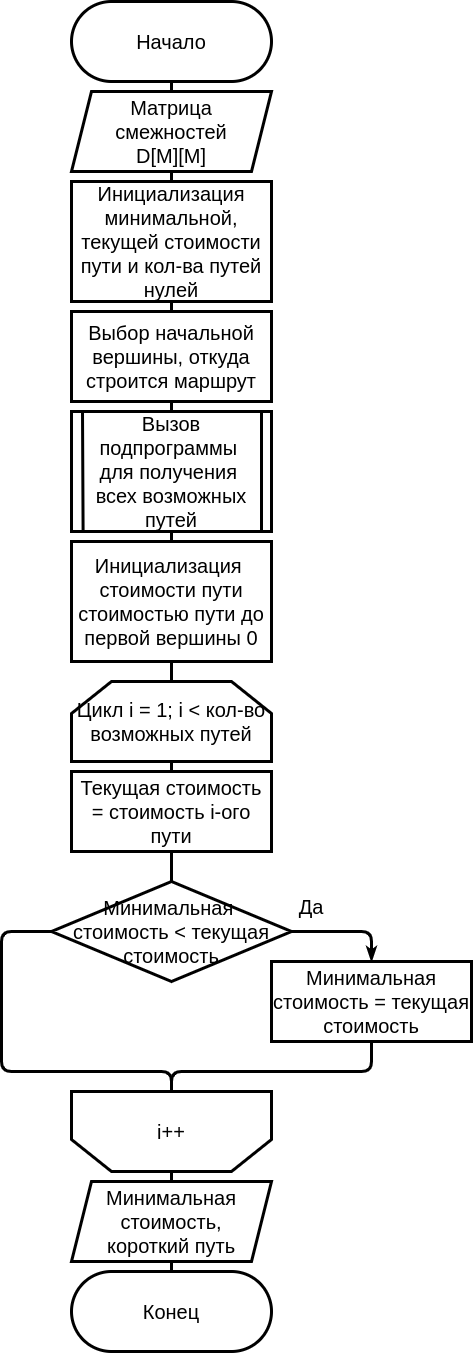
\includegraphics[scale=0.40]{l1.allsearch}}
  \caption{Схема алгоритма полного перебора}
  \label{ris:schemaposav}
\end{figure}

\subsection{Схема муравьиного алгоритма}\label{SchemaParRowMatrixMultiply}

На рисунке \ref{ris:schemaparrowav} показана схема муравьиного алгоритма.

\begin{figure}[H]
  \center{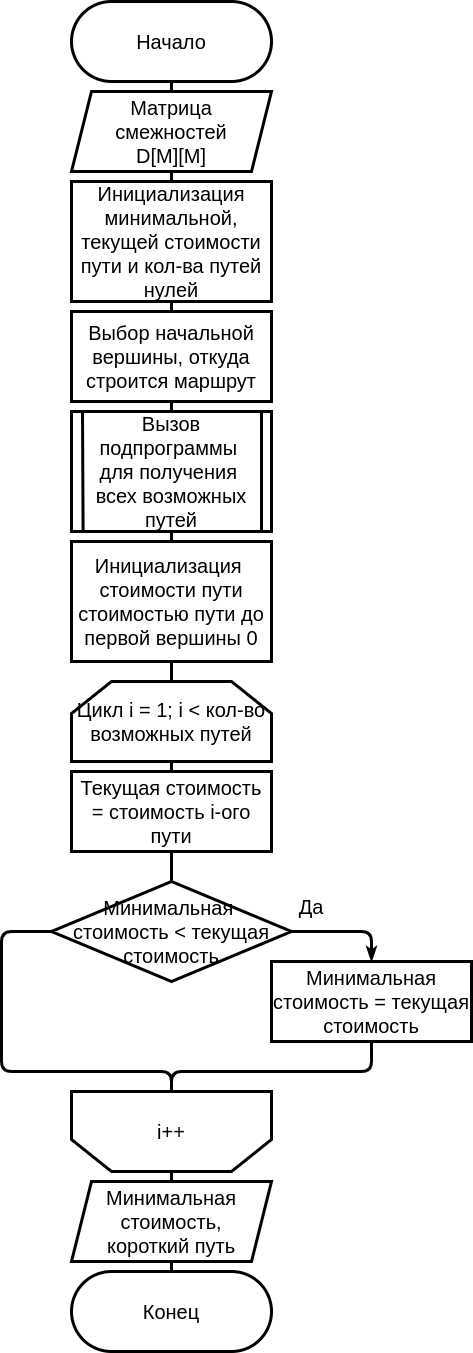
\includegraphics[scale=0.40]{l1.myravs}}
  \caption{Схема муравьиного алгоритма}
  \label{ris:schemaparrowav}
\end{figure}

%На рисунке \ref{ris:schemachoise} показана схема алгоритма сортировки выбором.

%\begin{figure}[H]
%  \center{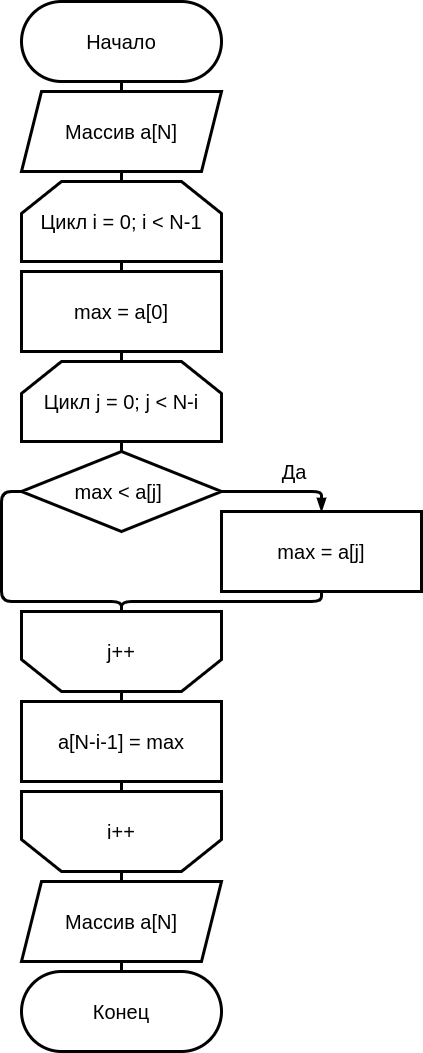
\includegraphics[scale=0.35]{l1.choise}}
%  \caption{Схема алгоритма сортировки выбором}
%  \label{ris:schemachoise}
%\end{figure}

%На рисунке \ref{ris:schemainsert} показана схема алгоритма сортировки вставками.

%\begin{figure}[H]
%  \center{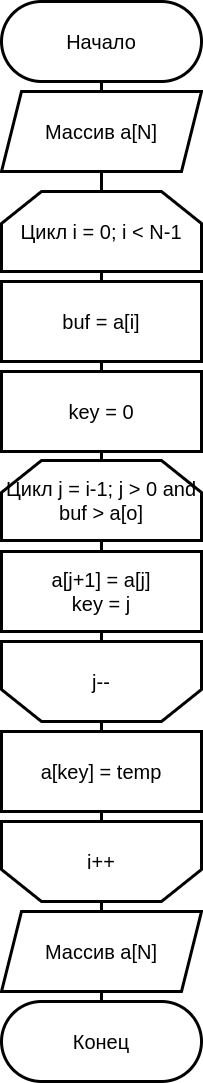
\includegraphics[scale=0.35]{l1.insert}}
%  \caption{Схема алгоритма сортировки вставками}
%  \label{ris:schemainsert}
%\end{figure}


\section{Структуры данных}\label{Structs}

При реализации приведенных алгоритмов потребуются типы данных: массив, матрица, муравей, колония.

\begin{enumerate}
  \item $D$ - матрица смежности
  \item $ Tao $ - матрица феромонов
  \item $\alpha$ - приоритет пути
  \item $\beta$ - приоритет феромона
  \item q - переносимый муравьем феромон
  \item p - коэффициент испарения 
  \item $t_{max}$ - максимальное время жизни колонии
\end{enumerate}

\section{Тестирование}\label{Testing}


Для алгоритма умножения матриц можно выделить следующие классы эквивалентности:

\begin{enumerate}
    \item ациклический ориентированный взвешенный граф;
    \item циклический ориентированный взвешенный граф.
\end{enumerate}

%\subsection{Способы тестирования}\label{TestingMethods}

%При разработке программы удобно использовать следующие методы тестирования:

%\begin{enumerate}
%    \item Модульные тесты 
%    \item Функциональные тесты 
%\end{enumerate}

\section{Вывод конструкторской части}\label{KonstructResult}
На основе данных, полученных в аналитическом разделе, были построены схемы используемых алгоритмов,
выделены необходимые для реализации структуры данных и методы тестирования.

